%%%%%%%%%%%%%%%%%%%%%%%%%%%%%%%%%%%%%%%%%%%%%%%%%%%%%%%%%%%%%%%%%%%%
% bare_jrnl.tex
% V1.4b
% 2015/08/26
% by Michael Shell
%%%%%%%%%%%%%%%%%%%%%%%%%%%%%%%%%%%%%%%%%%%%%%%%%%%%%%%%%%%%%%%%%%%%

\documentclass[journal]{IEEEtran}

\usepackage{instructivo}
\graphicspath{{./}{./fig/}}


\usepackage[natbib=true,style=trad-unsrt,backend=biber]{biblatex}
\usepackage{float}
\usepackage[section]{placeins}

\raggedbottom
\setlength{\textfloatsep}{8pt}
\setlength{\floatsep}{8pt}
\setlength{\intextsep}{8pt}

\addbibresource{literatura.bib}

% correct bad hyphenation here
\hyphenation{op-tical net-works semi-conduc-tor}

\begin{document}

\title{Proyecto: Semáforo vehicular y peatonal}

\author{Larry~Josué~Ramírez-Benavides,~\IEEEmembership{Estudiante,~ITCR} ,~Jose~Daniel~Villalobos-Monge,~\IEEEmembership{Estudiante,~ITCR,}  ~Esteban~Pérez-González,~\IEEEmembership{Estudiante,~ITCR,} y ~Maximiliano~Jesús~Jiménez-Jiménez,~\IEEEmembership{Estudiante,~ITCR,}
}

\markboth{EL3215 Laboratorio de Electrónica Analógica, IS2026}%
{EL3215 Laboratorio de Electrónica Analógica}

\maketitle

%%%%%%%%%%%%%%%%%%%%%%%%%%%%%%%%%%%%%%%%%%%%%%%%%%%%%%%%%%%%%%%%%%%%%%%%%%%%%%%%%%%%%%%%%%%%%%
\begin{abstract}

\end{abstract}

\begin{IEEEkeywords}

\end{IEEEkeywords}

%%%%%%%%%%%%%%%%%%%%%%%%%%%%%%%%%%%%%%%%%%%%%%%%%%%%%%%%%%%%%%%%%%%%%%%%%%%%%%%%%%%%%%%%%%%%%%
\section{Introducción}

\IEEEPARstart{E}{l} 

%%%%%%%%%%%%%%%%%%%%%%%%%%%%%%%%%%%%%%%%%%%%%%%%%%%%%%%%%%%%%%%%%%%%%%%%%%%%%%%%%%%%%%%%%%
\section{Resultados}

%%%%%%%%%%%%%%%%%%%%%%%%%%%%%%%%%%%%%%%%%%%%%%%%%%%%%%%%%%%%%%%%%%%%%%%%%%%%%%%%%%%%%%%%%
\subsection{Montajes empleados}


%%%%%%%%%%%%%%%%%%%%%%%%%%%%%%%%%%%%%%%%%%%%%%%%%%%%%%%%%%%%%%%%%%%
%%%%%%%%%%%%%%%%%%%%%%%%%%%%%%%%%%%%%%%%%%%%%%%%%%%%%%%%%%%%%%%%%%%
\FloatBarrier

\subsection{Datos experimentales y simulados}



%%%%%%%%%%%%%%%%%%%%%%%%%%%%%%%%%%%%%%%%%%%%%%%%%%%%%%%%%%%%%%%%%%%%%%%%%%%%%%%%%%%%
\FloatBarrier
\section{Conclusiones}



%%%%%%%%%%%%%%%%%%%%%%%%%%%%%%%%%%%%%%%%%%%%%%%%%%%%%%%%%%%%%%%%%%%%%%%%%%%%%%%%%%%%
\FloatBarrier
\section{Referencias}



%%%%%%%%%%%%%%%%%%%%%%%%%%%%%%%%%%%%%%%%%%%%%%%%%%%%%%%%%%%%%%%%%%%%%%%%%%%%%%%%%%%%
\FloatBarrier
\begin{IEEEbiography}[{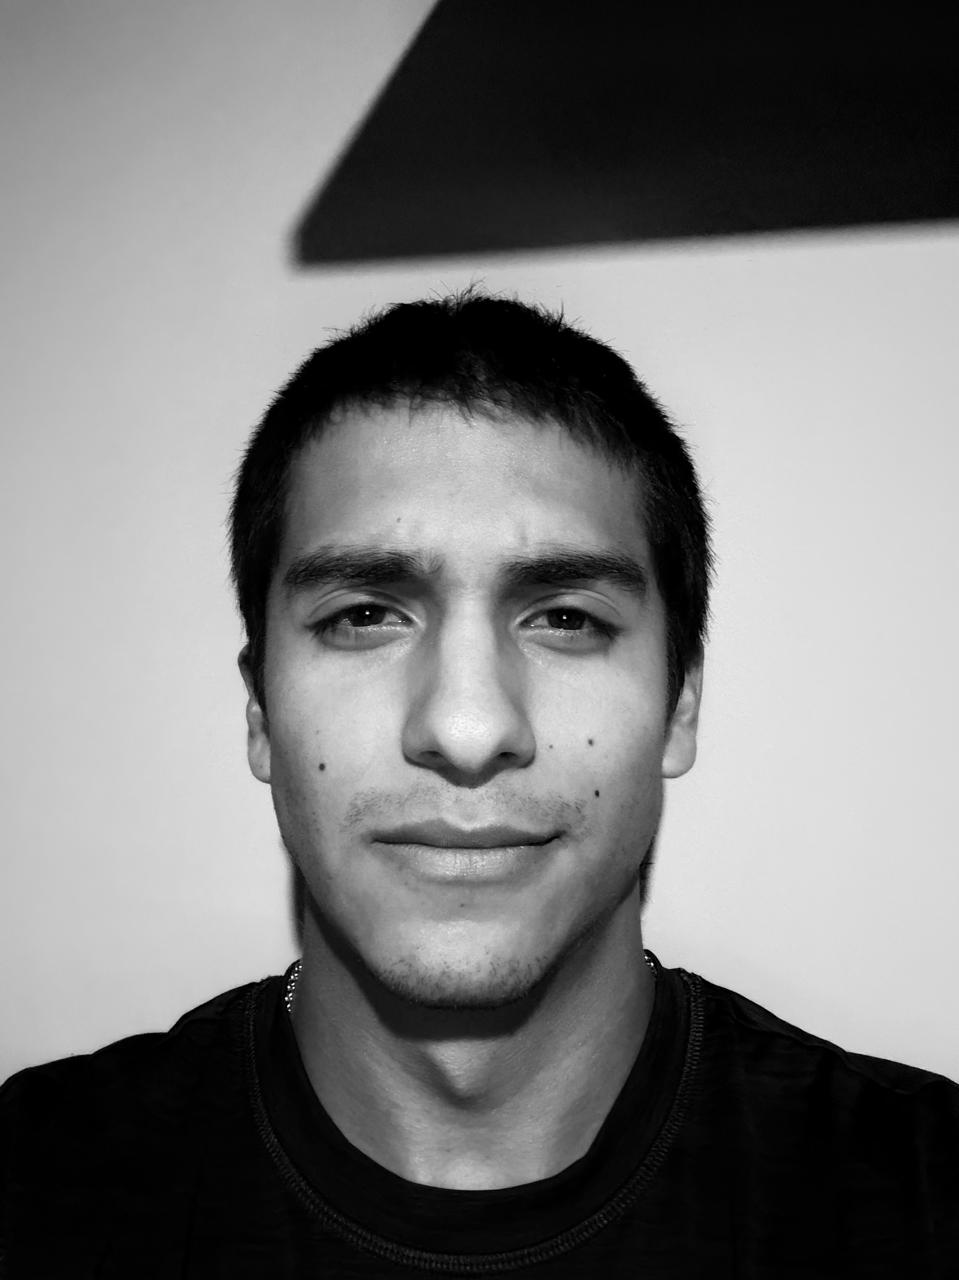
\includegraphics[width=1.05in,height=1.6in,clip,keepaspectratio]{fig/villalobos}}]{J. D. Villalobos Monge}

Nacido en Cartago, Costa Rica, el 9 de julio de 2004, realizó sus estudios de educación primaria y secundaria en el Colegio Anglo American. Posteriormente inició sus estudios universitarios en la carrera de Ciencias Actuariales en la Universidad de Costa Rica (UCR), donde cursó dos años. Actualmente se encuentra estudiando la carrera de Ingeniería Electrónica en el Instituto Tecnológico de Costa Rica (TEC), cursando su tercer año.

Cuenta con cuatro años de experiencia laboral en temporadas como asistente de administración en una Asociación Solidarista del Colegio Anglo American. Sus principales áreas de interés incluyen la robótica, los sistemas electrónicos y el desarrollo de vehículos eléctricos.

\end{IEEEbiography}

\begin{IEEEbiography}[{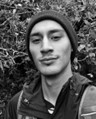
\includegraphics[width=1.05in,height=1.6in,clip,keepaspectratio]{ramirez}}]{L. J. Ramírez Benavides}

Nacido en Heredia, Costa Rica, el 28 de noviembre de 2004, obtuvo el título de Técnico en Electrónica Industrial en el Colegio Técnico Profesional de Zarcero en el año 2023. Actualmente cursa el tercer año de la carrera de Ingeniería Electrónica en el Instituto Tecnológico de Costa Rica (TEC).

Ha adquirido experiencia en el sector comercial a través de un negocio familiar y trabajó en Electrónica Zarcero antes de iniciar sus estudios universitarios. Sus principales áreas de interés incluyen los sistemas embebidos, el Internet de las Cosas (IoT) y la computación cuántica.

\end{IEEEbiography}

\vfill

\end{document}